%%%%%%%%%%%%%%%%%%%%%%%%%%%%%%%%%%%%%%%%%%%%%%%%%%%%%%%%%%%%%%%%%%%%%%%%%%%%%%%%%%%%%%%%%%%%%
%%									section 4.	Principe de Optimisation (α, \beta, \gamma)								%
%%%%%%%%%%%%%%%%%%%%%%%%%%%%%%%%%%%%%%%%%%%%%%%%%%%%%%%%%%%%%%%%%%%%%%%%%%%%%%%%%%%%%%%%%%%%%

\section{Principe d'Optimisation de $\alpha, \beta\; et\; \gamma$}
 
Dans le cas du model checking, les \'{e}tats pr\'{e}sentent des informations par rapport \`{a} la v\'{e}rification. L’analyse de ces r\'{e}sultats, montre que la distribution des \'{e}tats fortement li\'{e}s augmente le temps de traitement de la vérification, dans l'exemple pr\'{e}c\'{e}dant les \'{e}tats S1 et S5 sont li\'{e}s, leur distribution a augment\'{e} le temps de la vérification. Dans le cas d'un exemple plus complexe o\`{u} un ensemble d’\'{e}tats li\'{e}s sont distribu\'{e}s, le temps de la vérification sera très \'{e}lev\'{e}. L’id\'{e}e de faire basculés tous ces \'{e}tats dans une machine cela peut conduire \`{a} une centralisation de l'espace des états cela dégrade l'équilibrage de charge. L'optimisation des param\`{e}tres $\alpha, \beta \; et\; \gamma)$ revient \`{a} simuler un jeu coop\'{e}ratif entre les machines pour un but commun. 

La coop\'{e}ration des machines d\'{e}marre avec une prise de contact sur les valeurs initiales à savoir le nombre d’\'{e}tats stockés dans la machine et le nombre des états dupliqués de la \mi{} sur la \mj{}. A partir de ces valeurs il est possible de calculer le nombre minimum et maximum d’\'{e}tats qui sont susceptibles d’\^{e}tre stockés sur chaque machine. Le calcule de cette interval entre deux machines est comme suit :

\begin{itemize}
	\item  	On note $(\beta1 \; et\; \gamma1)$ les valeurs de la machine $M_1$ respectivement pour la machine $M_2$ $(\beta2 \;et\; \gamma2)$.
	\item  	On note $\overline{\beta}$ la moyenne des \'{e}tats $\overline{\beta}=\frac{\beta1+\beta2}{2}$.
	\item  	L’\'{e}cart type $\delta=\sqrt{\frac{\displaystyle\sum_{i=1}^{2}\beta_i^2 }{2}-\overline{\beta}^2} $
\end{itemize}

Par ailleurs le calcul de deux machines sont d\'{e}pendants par la présence des états successeurs  appartenant à des machines distantes, du fait de cette d\'{e}pendance certains \'{e}tats peuvent \^{e}tre fortement li\'{e}s, cela retarde la v\'{e}rification de la formule lorsqu'elle n'est pas vérifiée sur ces \'{e}tats. A titre d'exemple on a l'exemple précédent. Ainsi, lorsque la formule n'est pas vérifiée sur un \'{e}tat deux cas se présentent, soit elle n'est pas vérifiée sur l’\'{e}tat lui-m\^{e}me soit elle n'est pas vérifiée sur les successeurs de l'état, la réduction du temps de calcul$(\alpha)$ revient \`{a} chercher le nombre des \'{e}tats impliqu\'{e}s. La recherche des \'{e}tats liés peut \^{e}tre partagé en deux : 
\begin{itemize}
\item Sur la machine distante, l'algorithme recherche les états liés aux états qui n'appartiennent pas à la machine.
\item Sur la machine à laquelle l'état appartient, l'algorithme recherche les \'{e}tats pr\'{e}d\'{e}cesseurs liés à cet état. 
\end{itemize}
Ce parcours permet de retrouver les états qui peuvent être d\'{e}placés sur la machine. 


\begin{Exemple} 
Ce sc\'{e}nario est étudié sur l’exemple suivant:
   \centering
	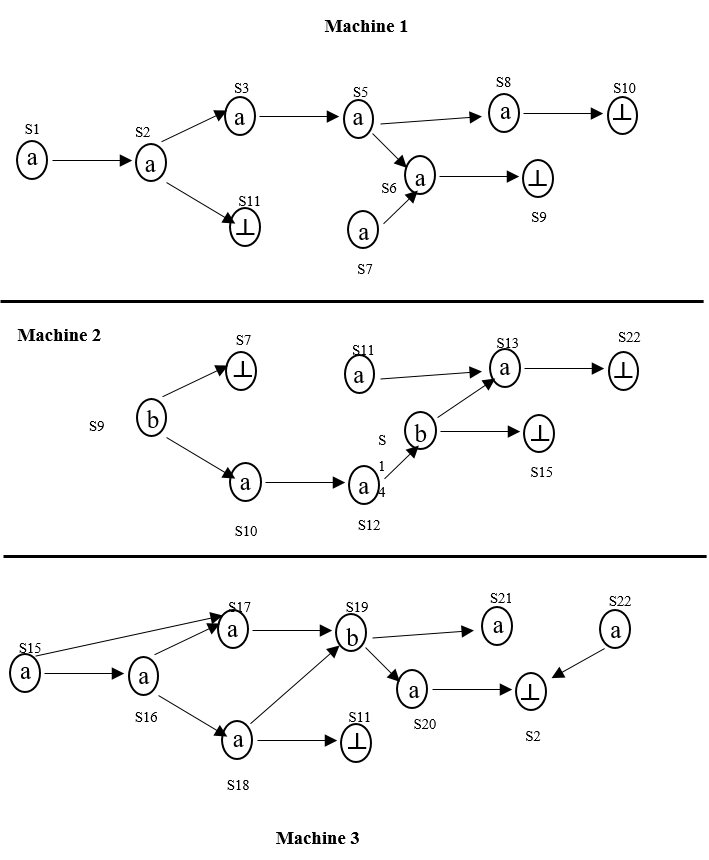
\includegraphics[height=4in]{img/skd2.png}	
	\captionof{figure}{Structure de kripke distribu\'{e}} \label{skd2}

\end{Exemple}